\documentclass[12pt]{beamer}
\usetheme{CambridgeUS}
\usepackage[utf8]{inputenc}
\usepackage{amsmath}
\usepackage{amsfonts}
\usepackage{color}
\usepackage{amssymb}
\author{Liujun Chen}
\title{Summary of 'Random threshold driven tail dependence measures with 
application to precipitation data analysis'}
%\setbeamercovered{transparent} 
%\setbeamertemplate{navigation symbols}{} 
%\logo{} 
%\institute{} 
%\date{} 
%\subject{} 
\begin{document}

\begin{frame}
\titlepage
\end{frame}

%\begin{frame}
%\tableofcontents
%\end{frame}

\begin{frame}{Tail dependence definition}
Two identically distributed random variables $X$ and $Y$ with distribution $F$ are called tail independent, if
\begin{displaymath}
\lambda=\lim_{u \to x_F} P(Y>u | X>u)
\end{displaymath}
exists and equal to 0, where $x_F=\sup \{ x\in \mathbb{R} :F(x)<1\}$. The quantity $\lambda$, if exists, is called the bivariate tail dependence index.
\end{frame}

\begin{frame}{Some Examples}
\begin{itemize}
\item The tail
dependence index of a bivariate normal (Gaussian) random vector is zero as long
as the corresponding correlation coefficient is less than one.
\item The tail dependence
index of a bivariate t random vector with a positive correlation is greater than
zero.
\end{itemize}
\begin{center}
{\color{blue}{\textbf{Dependent random variables are not necessarily tail dependent.}}}
\end{center}
\end{frame}

\begin{frame}{Focus of the Paper}
Two fundamental questions:
\begin{itemize}
\item How to identify tail dependencies between variables.
\item How to develop statistical models dealing with tail dependencies.
\end{itemize}
\vspace{3ex}
This paper is focus on the first issue.
\end{frame}

\begin{frame}{Hypotheses of tail independence}
\begin{center}
$\mathrm{H}_{0}: X$ and $Y$ are tail independent,

$\leftrightarrow H_{1}: X$ and $Y$ are tail dependent,
\end{center}
which can also be written as 
$$H_{0}: \lambda=0 \longleftrightarrow H_{1}: \lambda>0.$$

The remaining of the paper mainly discuss how to test the null and how to estimate $\lambda$ under the null hypothesis.
\end{frame}


\begin{frame}{Remarks of hypotheses of tail independence}
\begin{itemize}
\item The null and alternative hypotheses in Ledford and Tawn (1996,
1997) are reversed in this paper.
\begin{center}
$\mathrm{H}_{0}: X$ and $Y$ are tail dependent,

$\leftrightarrow H_{1}: X$ and $Y$ are tail independent.
\end{center}

\vspace{3ex}
\item Other significant tests include Falk and Michel(2006),Hüsler and Li (2009), Bacro, Bel, and Lantuéjoul (2010) etc.
\end{itemize}
\end{frame}

\begin{frame}{Tail independence test in Falk and Michel (2006)}
Let $\epsilon>0$ and $t\in [0,1]$. When $\epsilon$ tends to 0, the conditional distribution function
$$K_{\varepsilon}(t) \equiv P\left(X^{-1}+Y^{-1}<\varepsilon t | X^{-1}+Y^{-1}<\varepsilon\right)$$
tends to $t^2$ if $X$ and $Y$ are asymptotically independent, and t otherwise. This result can
be used to test for the asymptotic independence of X and Y using classical goodness-of-
fit tests such as the Kolmogorov–Smirnov or the likelihood ratio as well as the
chi-square test.
\end{frame}


\begin{frame}{Tail independence test in Hüsler and Li (2009) }
Assume some conditions, under $H_0$,
$$\mathrm{H}_{0}: l(x, y)=x+y \quad \text { for all } x, y>0,$$
it can be proved
$$\left\{T_{n}(x, y), x, y \in[0,1]\right\} \rightarrow\left\{W_{1}((1+\theta) x)+W_{2}((1+\theta) y), x, y \in[0,1]\right\},$$
where 
$$T_{n}(x, y):=\sqrt{k}\left(l_{n}(x, y)-(x+y)\right), \quad x, y \in[0,1],$$
and $W_1, W_2$ are independent Brownian motions.
\end{frame}
\begin{frame}{Tail independence test in Hüsler and Li (2009)-Continue }
And
$$\int_{0}^{1} \int_{0}^{1} k\left(l_{n}(x, y)-(x+y)\right)^{2} \mathrm{d} x \mathrm{d} y$$
$$ \quad \quad \quad  \stackrel{\mathrm{d}}{\rightarrow} \int_{0}^{1} \int_{0}^{1}\left(W_{1}((1+\theta) x)+W_{2}((1+\theta) y)\right)^{2} \mathrm{d} x \mathrm{d} y.$$
\end{frame}



\begin{frame}{Tail independence test in Bacro, Bel, and Lantuéjoul (2010)}
Consider the random variable 
\begin{displaymath}
W=\frac{1}{2}|F(X)-F(Y)|,
\end{displaymath}
it can be shown
$$\sqrt{n} \frac{\widehat{v_{W}}-\frac{1}{6}}{\widehat{\sigma_{W}}}\rightarrow  N(0,1),$$
where $\widehat{V_W}$ is an estimator for $E(W)$, and 
$\widehat{\sigma_W}$ is an estimator for $\sigma_W$. 
\end{frame}

\begin{frame}{TQCC and its properties}
\begin{itemize}
\item From the definition of $\lambda$, the estimation of $\lambda$ mainly relies on choice of thresholds $u$ the dependence mechanism between upper tails of
two random variables $X$ and $Y$.
\vspace{3ex}
\item This suggests that one can ignore values of $X$ and $Y$ below $u$ and construct sample-based measures of tail dependence.
\end{itemize}

\end{frame}


\begin{frame}{Definition of TQCC}
If $\left\{\left(X_{i}, Y_{i}\right)\right\}_{i=1}^{n}$ is a random sample of unit Fréchet random variables $(X,Y)$,
\begin{displaymath}
\mathrm{q}_{n, t}=\frac{\max _{i \leq n} \frac{\max \left(X_{i}, u_n\right)}{\max \left(Y_{i},u_n\right)}+\max _{i \leq n} \frac{\max \left(Y_{i}, u_n\right)}{\max \left(X_{i}, u_n\right)}-2}{\max _{i \leq n} \frac{\max \left(X_{i},u_n\right)}{\max \left(Y_{i}, u_n\right)} \times \max _{i \leq n} \frac{\max \left(Y_{i}, u_n\right)}{\max \left(X_{i}, u_n\right)}-1},
\end{displaymath}
is the tail quotient correlation coefficient(TQCC).

If $u_{n} \equiv u$, the TQCC reduces to the one in Zhang (2008). In this paper, $u_n$ is allowed to be random.
\end{frame}


\begin{frame}{Quotient correlation}
The quotient correlation, which can be used as an alternative to Pearson's correlation,is defined as 
\begin{displaymath}
\mathrm{q}_{n}=\frac{\max _{i \leq n}\left\{Y_{i} / X_{i}\right\}+\max _{i \leq n}\left\{X_{i} / Y_{i}\right\}-2}{\max _{i \leq n}\left\{Y_{i} / X_{i}\right\} \times \max _{i \leq n}\left\{X_{i} / Y_{i}\right\}-1}.
\end{displaymath}
Zhang(2008) proved that if $X$ and $Y$ are independent, then
\begin{displaymath}
n q_{n} \stackrel{\mathcal{L}}{\longrightarrow} \zeta,
\end{displaymath}
where $\zeta$ is a gamma(2, 1) random variable.
\end{frame}


\begin{frame}{Some properties of TQCC}
\begin{itemize}
\item Take $\zeta_{n}^{\mathrm{I}}=\max _{1 \leq i \leq n}\left\{\max \left(X_{i}, u_{n}\right) / \max \left(Y_{i}, u_{n}\right)\right\}$ and $\zeta_{n}^{\mathrm{II}}=\max _{1 \leq i \leq n}\left\{\max \left(Y_{i}, u_{n}\right) / \max \left(X_{i}, u_{n}\right)\right\}$.
\vspace{2ex}
\item Now $\mathrm{q}_{u_{n}}=f\left(\zeta_{n}^{\mathrm{I}}, \zeta_{n}^{\mathrm{II}}\right),$ where
\begin{displaymath}
f(x, y)=\frac{x+y-2}{x y-1}, \quad for x \geq 1, y \geq 1, x+y>2.
\end{displaymath}
\vspace{2ex}
\item It is easy to see that $0<f(x, y)<1, f(1, y)=1, f(x, 1)=1,$ and $\partial f / \partial x <0, \partial f / \partial y <0$.
\end{itemize}
\end{frame}




\begin{frame}{Some properties of TQCC-Continue}
The properties of $\mathrm{q}_{u_{n}}=f \left(\zeta_{n}^{\mathrm{I}}, \zeta_{n}^{\mathrm{II}}\right)$ can be summarised as follows.
\begin{itemize}
\item $\mathrm{q}_{u_{n}}$ takes values between 0 and 1
for a sufficiently large n.
\item For a fixed sample size n, the larger the $\zeta_{n}^{\mathrm{I}}$ or the $\zeta_{n}^{\mathrm{II}}$,the smaller
the $\mathrm{q}_{u_{n}}$,hence the less the agreement of changing magnitudes at tails.
\item As long as one of $\zeta_{n}^{\mathrm{I}}$ and $\zeta_{n}^{\mathrm{II}}$ is very large, $\mathrm{q}_{u_{n}}$ is largely determined by the smaller one.

\end{itemize}
\end{frame}


\begin{frame}{Proposition 1}
The tail dependence index $\lambda_{X,Y}$ of $X$ and $Y$ is equal to the tail dependence index $\lambda^*_{X,Y}$ of $\max \left(X, u_{n}\right)$ and $\max \left(Y, u_{n}\right)$ using a random threshold, $u_n=T_{n,t},$ where $T_{n,t}$ is a Fréchet variable with the distribution function $\exp \left(-n / x^{t}\right) \text { for } x>0, n \geq 0 \text { and } t>1.$
$$\lim _{u \rightarrow \infty} \frac{P(X>u, Y>u)}{P(X>u)}=\lim _{u \rightarrow \infty} \frac{P\left\{\max \left(X, T_{n, t}\right)>u, \max \left(Y, T_{n, t}\right)>u\right\}}{P\left\{\max \left(X, T_{n, t}\right)>u\right\}}.$$
\end{frame}


\begin{frame}{Main Assumption T1}
For $1<t<1+\delta,\delta>0,$ paired tail independent random variables $(X_i,Y_i)$ satisfy
$$\frac{\max _{1 \leq i \leq n} \max \left(X_{i}, T_{n, t}\right) / \max \left(Y_{i}, T_{n, t}\right)}{\max _{1 \leq i \leq n} \max \left(X_{i}, T_{n, t}\right) / T_{n, t}}=1+o_{p}(1),$$
\vspace{3ex}
$$\frac{\max _{1 \leq i \leq n} \max \left(Y_{i}, T_{n, t}\right) / \max \left(X_{i}, T_{n, t}\right)}{\max _{1 \leq i \leq n} \max \left(Y_{i}, T_{n, t}\right) / T_{n, t}}=1+o_{p}(1).$$
\end{frame}


\begin{frame}{Corollary 1}
If random variables $X_{1}, \ldots, X_{n}, Y_{1}, \ldots, Y_{n}$ satisfy T1, where $X_{i}$ and $Y_{i}$ -are unit Fréchet random variables, under the null hypothesis, 
$$2 n\left\{1-\exp \left(-\frac{1}{T_{n, t}}\right)\right\} \mathrm{q}_{T_{n, t}} \stackrel{\mathcal{L}}{\rightarrow} \chi_{4}^{2},$$
where $\chi_{4}^{2}$ is a chi-squared random variable with four degrees of freedom.
\end{frame}

\begin{frame}{Corollary 2}
If random variables $X_{1}, \ldots, X_{n}, Y_{1}, \ldots, Y_{n}$ satisfy T1,and
$u_{n}=u_{n}^{*} a_{n}$ satisfies $u_{n}^{*} \stackrel{\mathrm{P}}{\rightarrow} u^{*}, a_{n} \rightarrow \infty,$ and $a_{n} / n \rightarrow 0$ as $n \to \infty$, where $X_{i}$ and $Y_{i}$ -are unit Fréchet random variables, under the null hypothesis, 
$$2 n\left\{1-\exp \left(-1 / u_{n}\right)\right\} \mathrm{q}_{u_{n}} \stackrel{\mathcal{L}}{\rightarrow} \chi_{4}^{2}.$$
\end{frame}


\begin{frame}{Condition A1}
Let $\left\{\xi_{i, j}: i \geq 1,-\infty<j<\infty\right\}$ be mutually independent unit Fréchet random variables, and suppose that tail dependent unit Fréchet random variables $X_i$ and $Y_i$ have the approximation representations
$$X_{i}=\max _{-\infty<j<\infty} \alpha_{j} \xi_{i, j}, \quad Y_{i}=\max _{-\infty<j<\infty} \beta_{j} \xi_{i, j},$$
where $\alpha_{j} \geq 0, \beta_{j} \geq 0, \sum_{j=-\infty}^{\infty} \alpha_{j}=1, \sum_{j=-\infty}^{\infty} \beta_{j}=1,$ and $\alpha_{j}>0$ iff $\beta_{j}>0$ for all j. Then there exist 
$0<c_1<c_2<\infty$ such that $c_1\le \alpha_j/\beta_j \le c_2$.
\end{frame}

\begin{frame}{Theorem 5}
Suppose that $\left\{X_{i}\right\}_{i=1}^{n}$ and $\left\{Y_{i}\right\}_{i=1}^{n}$ satisfy A1. Then for $u_n=T_{n,t}\stackrel{P}{\to} \infty$ in Theorem 3, and $u_{n}=u_{n}^{*} a_{n}$ with $u_{n}^{*} \stackrel{\mathrm{P}}{\rightarrow} u^{*} \in(0, \infty), a_{n} \rightarrow \infty$ and
$a_n/n\to 0$ in Theorem 4, $2 n\left\{1-\exp \left(-1 / u_{n}\right)\right\} \mathrm{q}_{u_{n}} \stackrel{\mathrm{P}}{\rightarrow} \infty$, and the test is consistent.
\end{frame}

\begin{frame}{Proposition 3}
Suppose $\alpha_{1}+\alpha_{2}=1$ and $\beta_{1}+\beta_{2}=1$. Then $\mathrm{q}_{u_{n}} \stackrel{\mathrm{P}}{\rightarrow} \lambda.$
\end{frame}

\begin{frame}{Marginal Transformation}
The GEV has the form
\begin{displaymath}
H(x ; \xi, \mu, \psi)=\exp \left[-\left\{1+\frac{\xi(x-\mu)}{\psi}\right\}_{+}^{-1 / \xi}\right].
\end{displaymath}
In principle, unit Fréchet scales can be obtained using the transformation $-1 / \log \{H(x ; \xi, \mu, \psi)\}.$
\end{frame}



\begin{frame}{Theorem 4}
Let $\left\{\left(X_{i}, Y_{i}\right)\right\}_{i=1}^{n}$ be a sample of $T1$ type tail independent random variables $(X,Y)$ whose marginal domains of attraction are GEV random variables with shape parameters $\xi_{X}=\xi_{0 ; X}$ and $\xi_{Y}=\xi_{0 ; Y},$ respectively. Suppose estimators of $\xi_{X}$ and $\xi_{Y}$, satisfy $n^{\alpha_{X}}\left(\hat{\xi}_{X}-\xi_{0 ; X}\right) \stackrel{\mathcal{L}}{\rightarrow} W_{X}$ and $n^{\alpha_{Y}}\left(\hat{\xi}_{Y}-\xi_{0 ; Y}\right) \stackrel{\mathcal{L}}{\rightarrow} W_{Y},$ where $\alpha_{X}>0$, $\alpha_{Y}>0$ and $W_{X}$ and $W_{Y}$ are random variables. If $\hat{X}_{i}=-1 / \log \left\{H\left(X_{i} ; \hat{\xi}_{X}\right)\right\}, \hat{Y}_{i}=-1 / \log \left\{H\left(Y_{i} ; \hat{\xi}_{Y}\right)\right\}$ and
$\hat{\mathrm{q}}_{u_{n}}=\frac{\max _{1 \leq i \leq n}\left\{\max \left(\hat{X}_{i}, u_{n}\right) / \max \left(\hat{Y}_{i}, u_{n}\right)\right\}+\max _{1 \leq i \leq n}\left\{\max \left(\hat{Y}_{i}, u_{n}\right) / \max \left(\hat{X}_{i}, u_{n}\right)\right\}-2}{\max _{1 \leq i \leq n}\left\{\max \left(\hat{X}_{i}, u_{n}\right) / \max \left(\hat{Y}_{i}, u_{n}\right)\right\} \times \max _{1<i \leq n}\left\{\max \left(\hat{Y}_{i}, u_{n}\right) / \max \left(\hat{X}_{i}, u_{n}\right)\right\}-1}$, then
$$ 2 n\left\{1-\exp \left(-1 / u_{n}\right)\right\} \hat{\mathrm{q}}_{u_{n}} \stackrel{\mathcal{L}}{\rightarrow} \chi_{4}^{2}.$$
\end{frame}


\begin{frame}{Data Application}
\begin{itemize}
\item The data are daily precipitation totals covering the period 1950-1999 over 5873 stations in the continental USA.
\item Fit GEV to each of 5,873 series, performed marginal transformations, conduct TQCC-based tail independence tests, and report the tail dependence measure (TQCC) after controlling the false discover rate (FDR) at level 0.05.
\end{itemize}
\end{frame}

\begin{frame}{GEV fitting and extreme precipitation comparison}
Table 1. Information of six selected stations. The top three stations have smallest $\hat{\epsilon}$, and the bottom three have the largest.
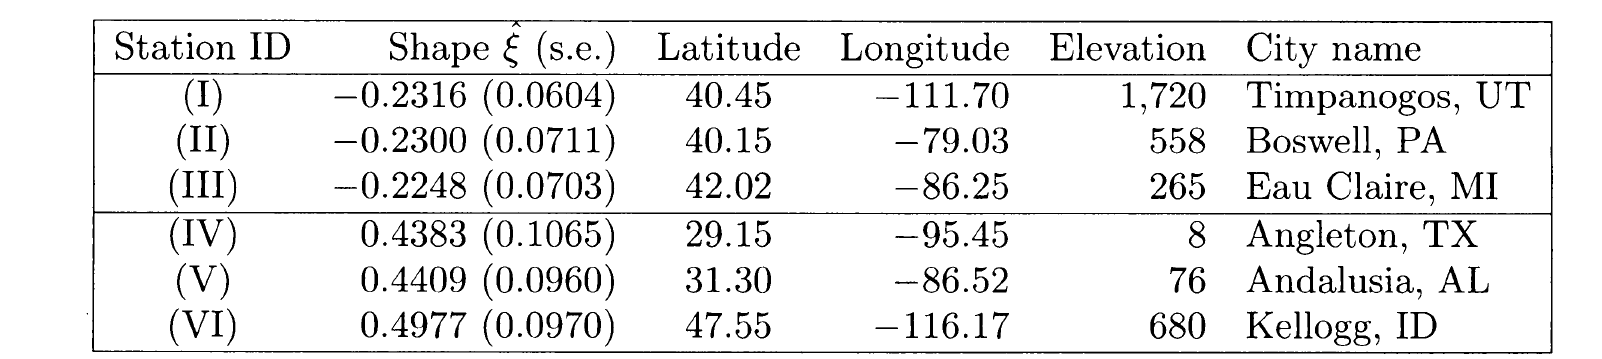
\includegraphics[scale=0.7]{figure1.png}
\end{frame}

\begin{frame}{GEV fitting and extreme precipitation comparison}
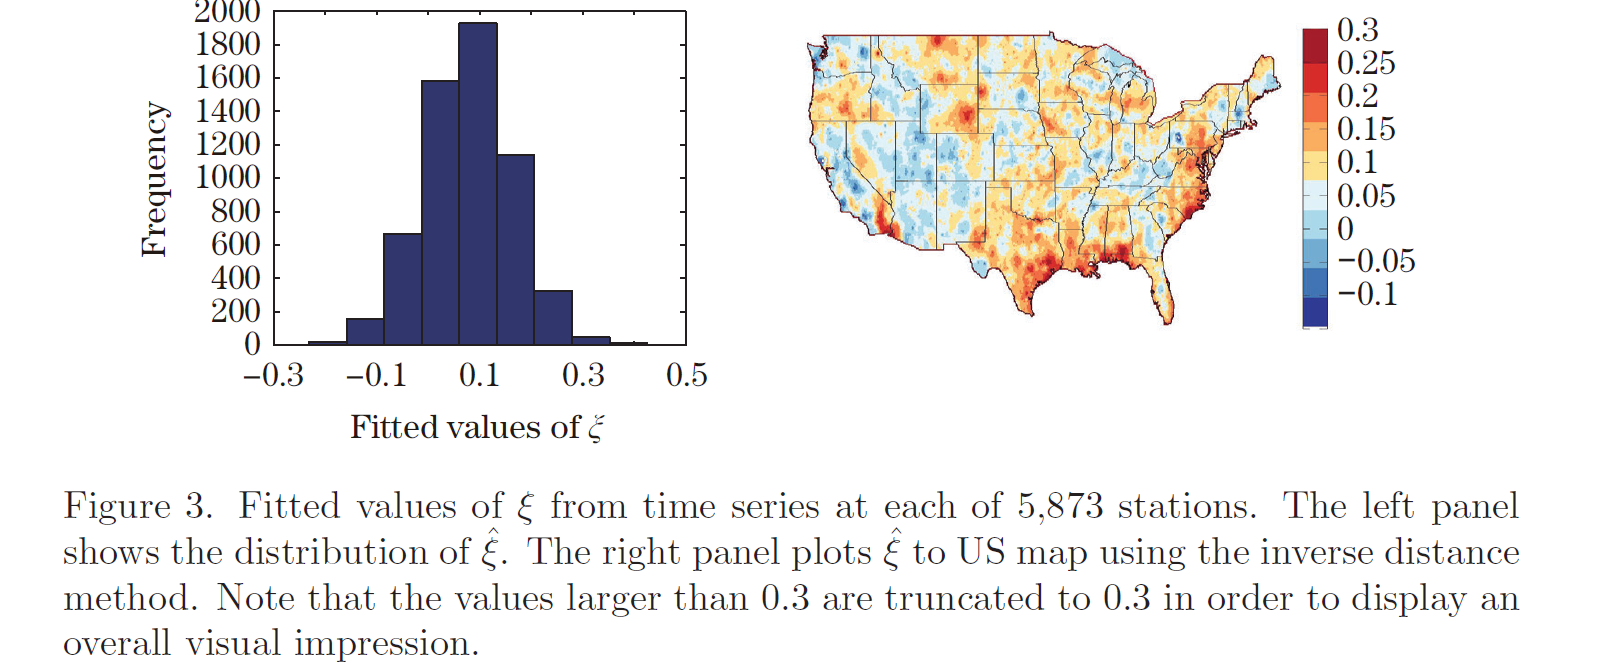
\includegraphics[scale=0.7]{figure2.png}
\end{frame}


\begin{frame}{Overall tail dependency across all stations}
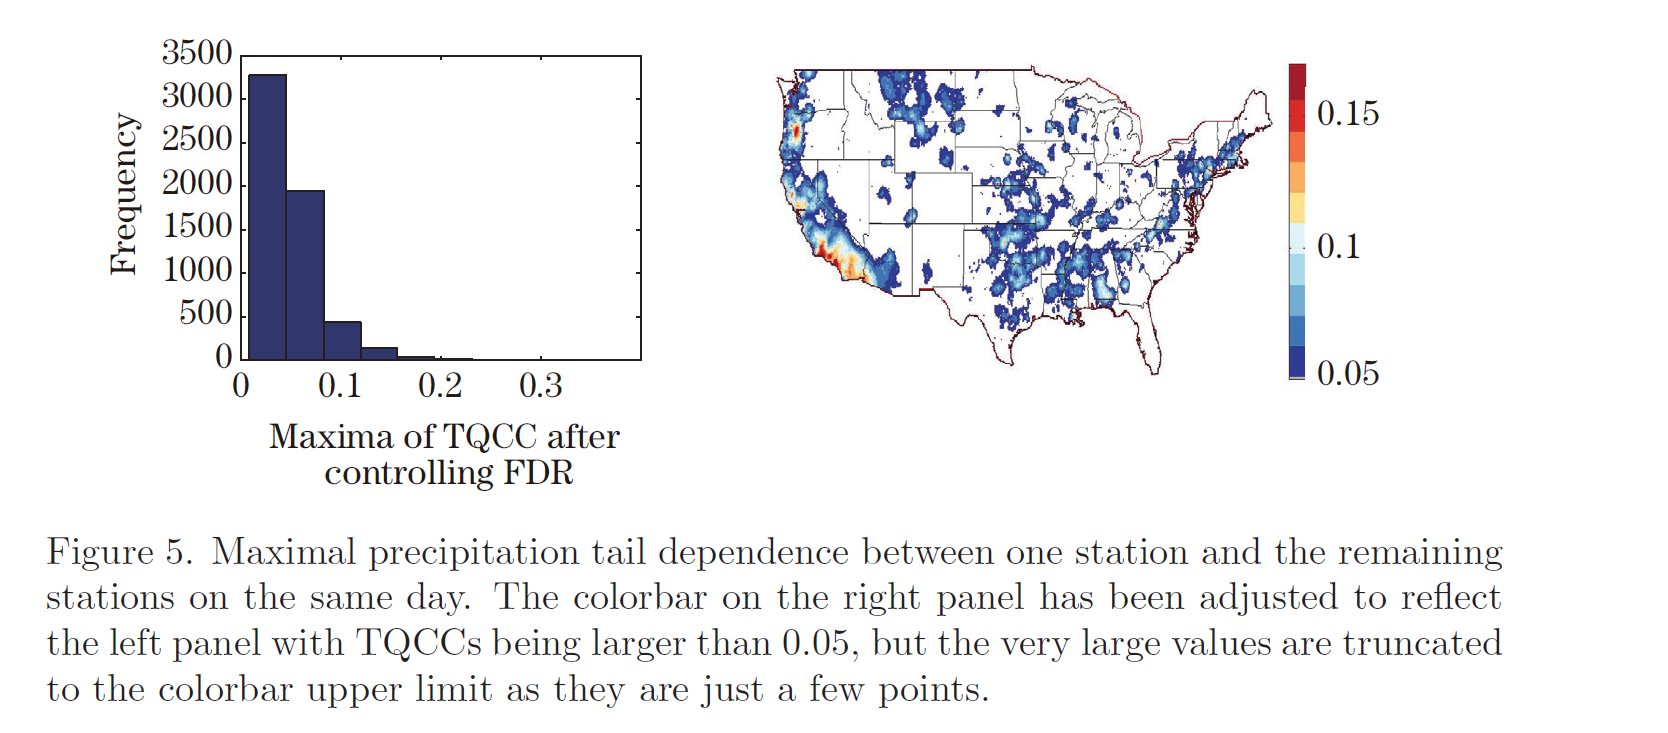
\includegraphics[scale=0.7]{figure3.png}
\end{frame}
\begin{frame}{Overall tail dependency across all stations}
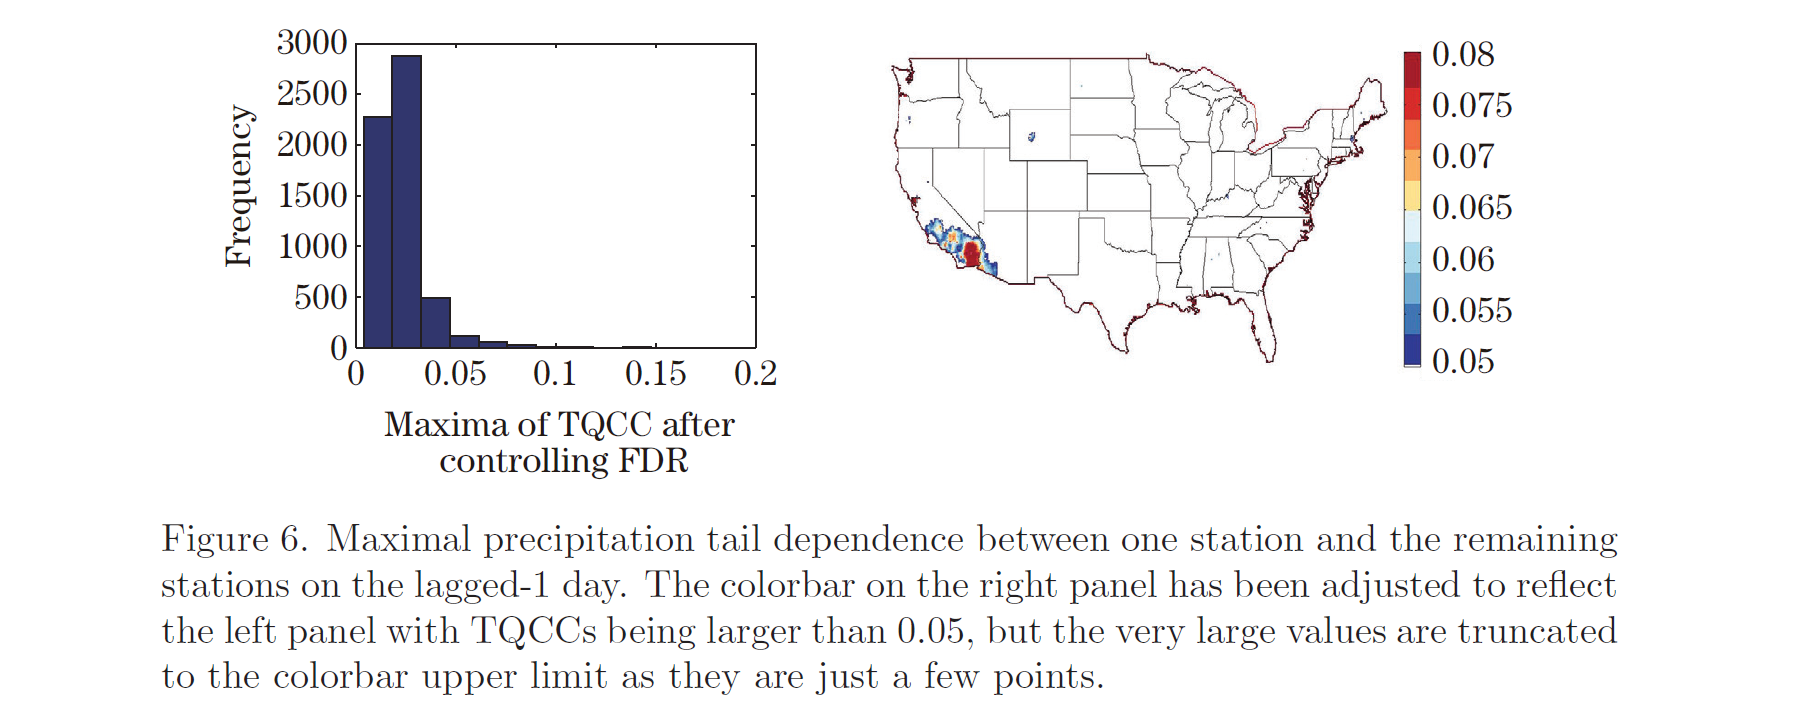
\includegraphics[scale=0.7]{figure4.png}
\end{frame}
\begin{frame}{Overall tail dependency across all stations}
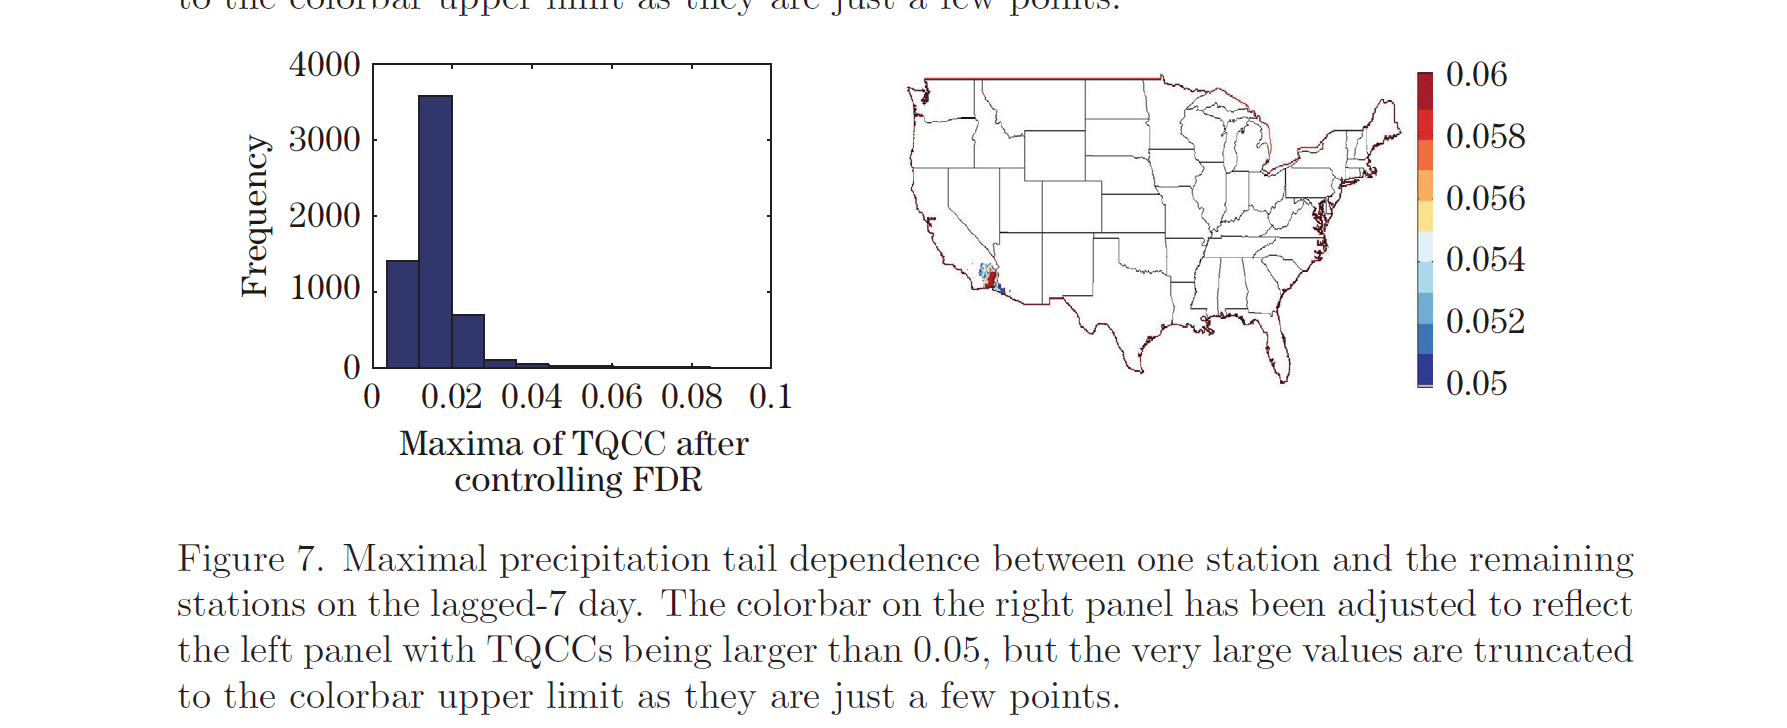
\includegraphics[scale=0.7]{figure5.png}
\end{frame}
\end{document}
